\documentclass[acmtog, screen]{acmart}

\usepackage[utf8]{inputenc}
\usepackage[spanish]{babel}
\usepackage{graphicx}
\graphicspath{{../fig/}}

\usepackage{booktabs} % For formal tables
\usepackage{hyperref}
\usepackage{amsmath}

% Document starts
\begin{document}
% Title portion
\title{Desarrollo de Sistemas Inteligentes - Trabajo de predicción}

\author{Luis Cabañero Gómez}
\email{Luis.Cabanero@alu.uclm.es}

\maketitle

Enlace a repositorio GitHub: \url{https://github.com/Xiul109/DSI}

Enlace a vídeo de Youtube: \url{https://www.youtube.com/watch?v=o6bFHeahwb8}

Enlace al usuario de DrivenData: \url{https://www.drivendata.org/users/xiul/}

\section{Introducción}
Este documento describe el proceso que se ha seguido para intentar predecir el número de casos de dengue a partir de los datos de la competición \href{https://www.drivendata.org/competitions/44/dengai-predicting-disease-spread/page/80/}{DengAI} de DrivenData. Se ha utilizado Python como lenguaje de programación para crear el modelo y realizar la predicción. Además, se han utilizado las siguientes librerías:
\begin{itemize}
	\item \textbf{NumPy}: Para trabajar con matrices y realizar algunas operaciones y transformaciones.
	\item \textbf{pandas}: Para cargar y guardar los ficheros .csv, así como para trabajar de manera más cómoda con los datos ya cargados.
	\item \textbf{scikit-learn:} Se han utilizado funcionalidades de esta librería para llevar a cabo la validación cruzada.
	\item \textbf{Keras:} Para construir los modelos de redes neuronales. Keras permite simplificar el uso de otras librerías útiles para crear redes neuronales, permitiendo un nivel de abstracción mayor. Como backend se ha utilizado \textbf{TensorFlow}, que es la opción que da por defecto.
\end{itemize}

Se han llevado a cabo diversas aproximaciones para intentar solucionar el problema con la mejor puntuación posible, sin embargo muchas han conseguido lo contrario. La puntuación más alta conseguida ha sido 25.2188  y en este documento se describirán primero los procesamientos y el modelo que han servido para obtener esta puntuación. Después se tratarán las aproximaciones fallidas y las conclusiones extraídas.

\section{Acercamiento inicial al problema}
Tras leer la descripción del problema se tuvieron dos ideas iniciales sobre cómo afrontarlo:
\begin{itemize}
	\item \textbf{Entrenar dos modelos.} Teniendo en cuenta que hay dos ciudades y que las condiciones son diferentes en cada una, se ha creído conveniente crear un modelo para cada ciudad. Investigando diferentes acercamientos de otras personas que han participado en la competición, se ha comprobado que crear un modelo por ciudad es algo habitual.
	\item \textbf{Tener en cuenta el carácter temporal de los datos.} Al tratarse de series temporales y teniendo en cuenta de que el tiempo desde que ponen huevos los mosquitos hasta que crece un mosquito adulto nuevo pasa en torno a 2 o 3 semanas, se pensó que sería positivo para la predicción tener en cuenta los datos de semanas previas. Sin embargo, se probaron varios acercamientos para tener en cuenta la temporalidad de los datos(de los que se hablará posteriormente) y ninguno de ellos contribuyó a mejorar los resultados.
\end{itemize}

Para tener una primera toma de contacto con los datos no se ha escrito ningún script ni se ha utilizado ninguna herramienta específica, sino que se ha leído \href{http://drivendata.co/blog/dengue-benchmark/}{esta entrada} en el blog de DrivenData en la que se hace un análisis exploratorio de los datos y se entrena a un modelo de prueba. En este análisis muestran que ninguna variable por si sola está fuertemente relacionada con el número de casos en ninguna de las ciudades y también se ve cómo están correlacionadas las diferentes variables entre sí. Las variables con más correlación con el número de casos en ambas ciudades son indicadores de humedad, seguidas por variables de temperatura. Otra cosa que también se ve en en análisis es que faltan valores, por lo que es necesario tenerlo en cuenta.

Las figuras \ref{fig:casosIquitos} y \ref{fig:casosSanJuan} muestran la evolución temporal para las ciudades de Iquitos y San Juan respectivamente. En ellas se puede ver que, aunque hay bastante variabilidad, también tienen cierta tendencia periódica.

\begin{figure}[h]
	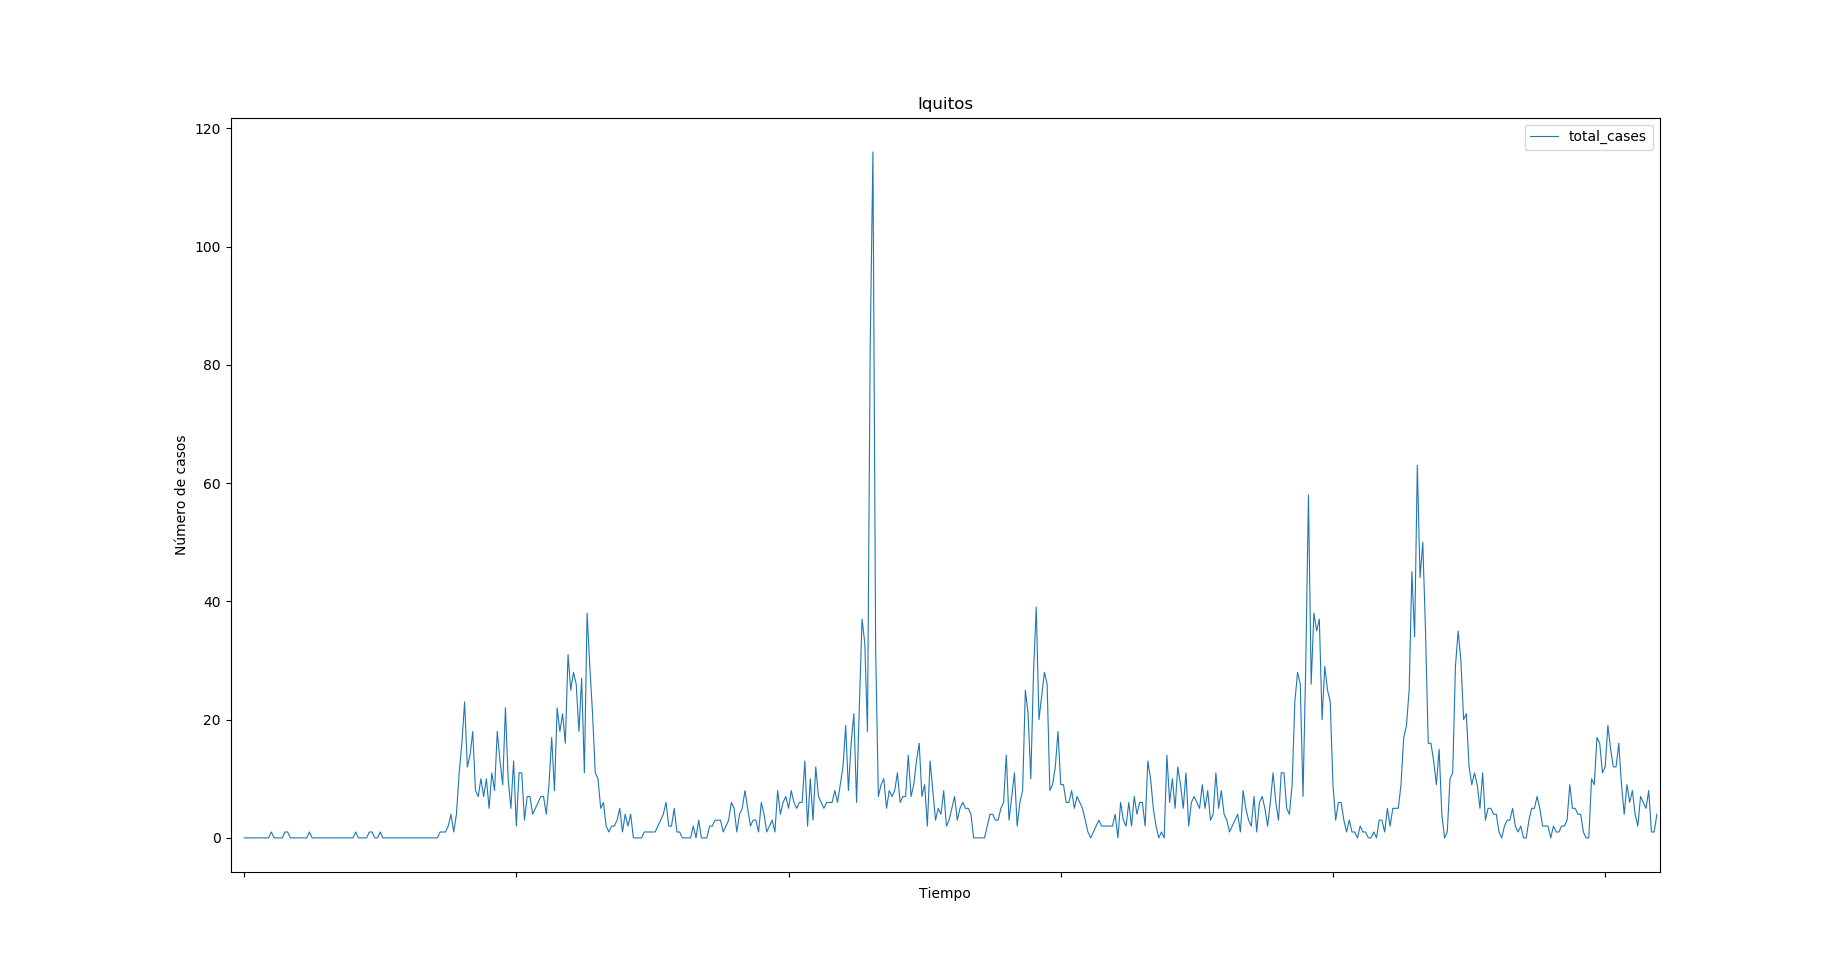
\includegraphics[width=\columnwidth]{casosIquitos}
	\caption{Evolución temporal del número de casos para la ciudad de Iquitos.}
	\label{fig:casosIquitos}
\end{figure}
\begin{figure}[h]
	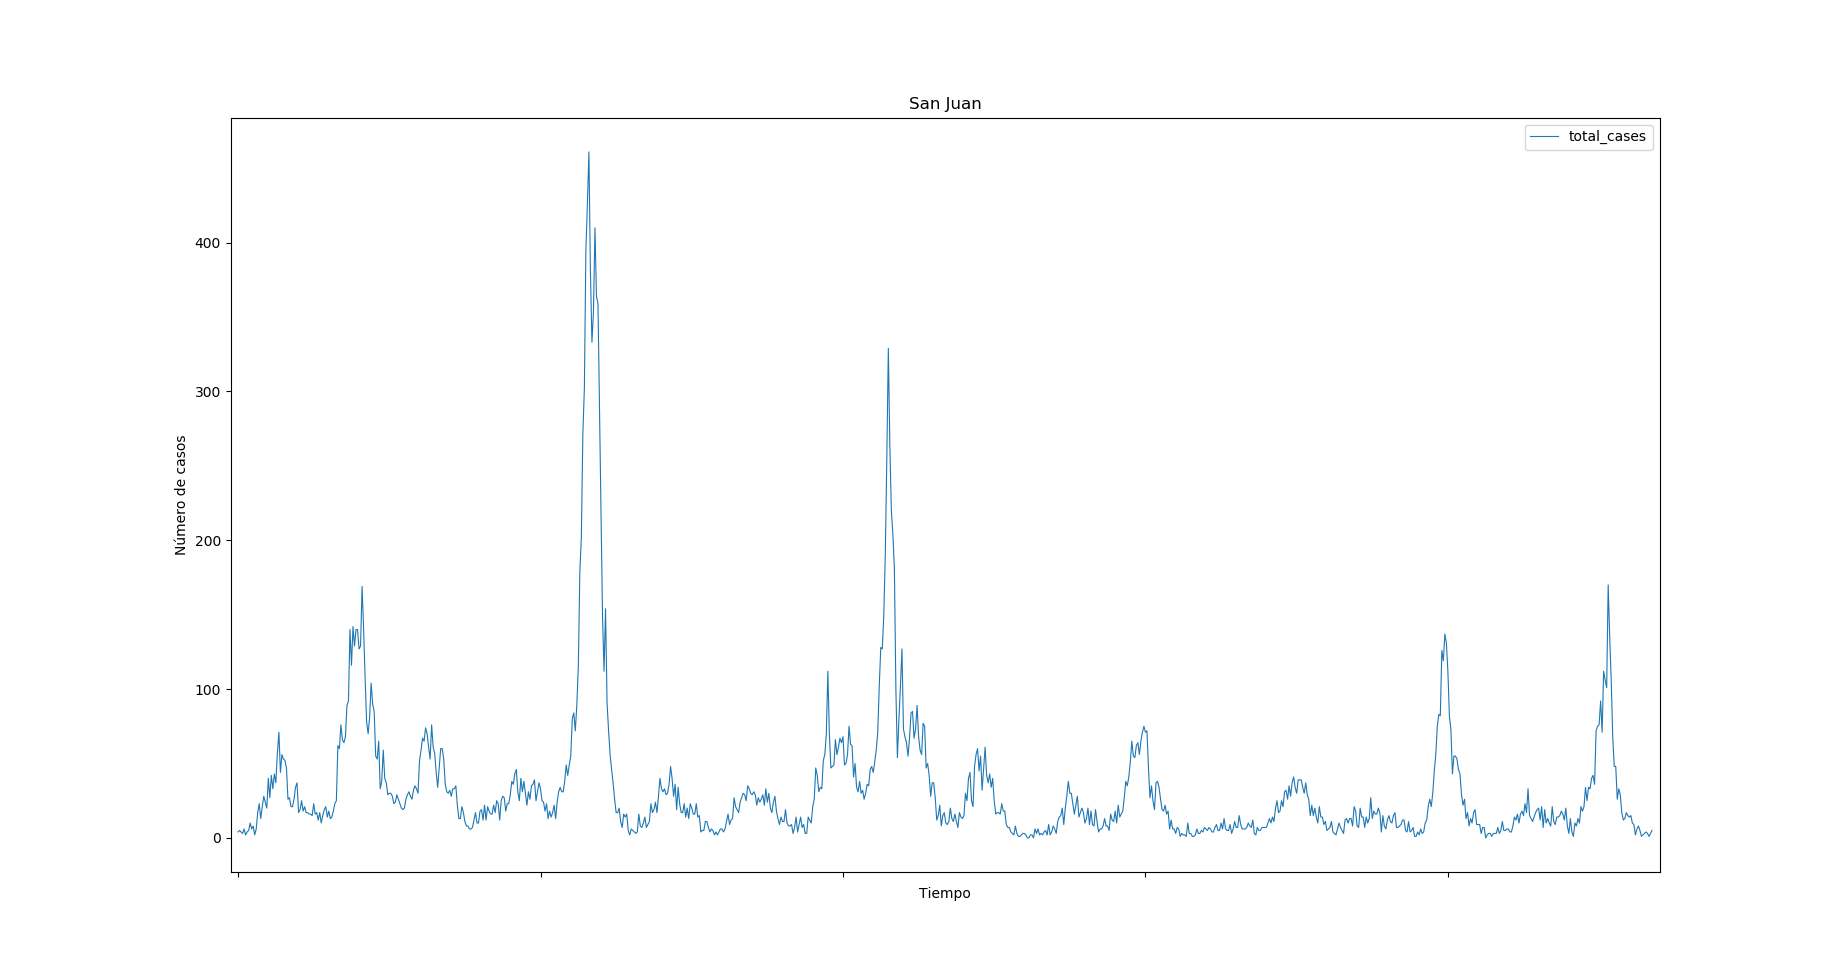
\includegraphics[width=\columnwidth]{casosSanJuan}
	\caption{Evolución temporal del número de casos para la ciudad de San Juan.}
	\label{fig:casosSanJuan}
\end{figure}

\section{Código}
El código que se ha utilizado consta de tres ficheros diferentes (aunque hay otro más relativo a una de las aproximaciones fallidas del que se hablará luego):
\begin{itemize}
	\item \textbf{funciones.py}: En este fichero se incluyen una serie de funciones que se llamarán desde los otros dos. La finalidad de sacar las funciones a otro fichero es poder aligerar y facilitar la comprensión de los otros dos.
	\item \textbf{validacion.py}: En este fichero se realizan una serie de pruebas mediante la técnica de validación cruzada con el fin de evaluar la eficacia del modelo. Esta medida de eficacia tiene un carácter bastante orientativo, ya que mejores resultados de la validación no significaban necesariamente mejores resultados con los datos de prueba.
	\item \textbf{prediccion.py}: En este fichero se entrena un modelo por ciudad, se intentan predecir los casos de dengue a partir de los datos de prueba y se genera el fichero .csv preparado para poder ser mandado a la competición.
\end{itemize}
La estructura tanto del fichero de predicción como la del fichero de validación sigue un patrón similar:

Primero se cargan los datos de entrenamiento con una función creada para ese fin, la cual permite seleccionar mediante parámetros con qué campos se queda o qué campos excluye. Esta función, además trata las filas con datos faltantes obteniendo estos mediante interpolación linear, lo cual se realiza mediante el método interpolate de los objetos de la clase DataFrame de la librería pandas.

Después se crea un objeto StandardScaler de scikit-learn que permite escalar los valores mediante la técnica de Z-Scores. Ese objeto se utiliza para escalar los valores de entrada de los datos y se almacena para, en el caso del script de predicción, utilizarlo luego para los datos de prueba.

A continuación se define el modelo para lo cual se ha creado una función que construye el modelo de una forma específica en base a los siguientes parámetros:
\begin{itemize}
	\item \textbf{nCols}: El número de características, la cual será equivalente al número de neuronas de la capa de entrada.
	\item \textbf{hiddenLayers:} Número de capas ocultas.
	\item \textbf{fUnits:} Una función para generar la cantidad de neuronas de una capa, la cual es útil para definir la topología de la red neuronal y espera recibir tres parámetros: el número de características, el número de capas ocultas y la posición de la capa. Se han definido dos de estas funciones para probar diferentes topologías:
	\begin{itemize}
		\item \textbf{uniforme}: Esta función genera topologías con capas que tienen siempre la misma cantidad de neuronas.
		\item \textbf{embudo}: Esta función genera topologías en las que cada capa tiene menos neuronas que la anterior. Haciendo algunas pruebas con ambas topologías han mostrado resultados similares.
	\end{itemize}
	En cuanto a la capa de salida siempre se generaba con una sola neurona.
	\item \textbf{lr}: Este es el ratio de aprendizaje, es decir, cuánto se modifican los pesos con cada ejemplo que se le pasa a la red.
	\item \textbf{decay:} Este es el ratio de aprendizaje e afecta a cuanto se reduce el ratio de aprendizaje en cada época siguiendo la siguiente ecuación: $lr' = lr \cdot \dfrac{1}{1+decay*iteration}$ .
\end{itemize}
La librería Keras permite elegir qué algoritmo de optimización, que función hay que optimizar y la función de activación de las neuronas. En este caso, como algoritmo de optimización se ha utilizado Adam, ya que, tras hacer una breve investigación se ha determinado que funciona bastante bien. En cuanto a la función a optimizar, se ha utilizado el error absoluto medio, ya que al final es la que se evalúa en la competición. La función de activación que se ha utilizado es ReLU, la cual se define como $ReLU(x) = max(0,x)$ y en este caso se ha considerado que es la más útil ya que genera salidas estrictamente positivas y no acotadas a un rango específico.

A partir de aquí los scripts de predicción y de validación difieren un poco más. En ambos se llaman a funciones que toman muchos parámetros en común: las características para cada semana, el número de casos para cada semana, la función para construir el modelo y el número de épocas. 

La función de validación, se llama a una función llamada validacion\_cruzada y, además de los parámetros anteriormente descritos, tiene uno más: la cantidad de particiones a hacer para la validación. Esta función tiene en cuenta que se están usando series temporales, por lo que se utiliza el objeto TimeSeriesSplit de scikit-learn para hacer las divisiones en lugar del objeto KFold. Esta función muestra por pantalla la media y la desviación típica del error medio absoluto para cada ejecución. El script de validación acaba aquí.

En el caso del script de predicción se llama a la función entrenar\_regresor, la cual devuelve un regresor entrenado con los parámetros que se le ha proporcionado. A continuación se cargan los datos de test y se llama a la función predecir\_casos, que toma como parámetros el regresor ya entrenado, los datos de prueba y un objeto Scaler para normalizar esos datos y devuelve el número de casos predichos para cada fila de los datos de prueba (la salida de la red se redondea para obtener el resultado en números enteros). Por último, se juntan los datos de Iquitos y San Juan y se genera el fichero .csv que se subirá a la web de la competición para ser evaluado.

\section{Mejor resultado}
Para llegar al mejor resultado que se ha alcanzado se han tenido en cuenta los siguientes puntos:
\begin{itemize}
	\item \textbf{Selección de características}: Se han seleccionado las características que identificaban más relevantes en la entrada del blog que se ha enlazado previamente: 'station\_avg\_temp\_c', 'station\_min\_temp\_c', 'reanalysis\_specific\_humidity\_g\_per\_kg' y 'reanalysis\_dew\_point\_temp\_k'. En adición a esas características, se ha añadido la semana, ya que parece que define cierta tendencia cíclica en el número de casos. Se han hecho pruebas usando muchas más características, pero eso solo llevaba a una situación de sobre-aprendizaje y, por lo tanto, peores resultados.
	\item \textbf{Topología}: La función usada para definir la topología es la función embudo y el número de capas ocultas es igual al doble de características seleccionadas (en este caso 10). Esto genera una topología que empieza con 10 neuronas en la primera capa oculta y se va reduciendo linealmente hasta llegar a 1 neurona en la última capa oculta.
	\item \textbf{Entrenamiento}: Para el entrenamiento se han utilizado 1500 épocas, un ratio de aprendizaje inicial de 0.05 y un ratio de decaimiento de 0.005. Para seleccionar estos parámetros se ha hecho de manera experimental teniendo en cuenta dos aspectos: la convergencia del modelo y los resultados que proporcionaba el mismo. En la figura \ref{fig:lossIquitos} se puede ver la evolución del aprendizaje de la red para la ciudad de Iquitos y en la figura \ref{fig:lossSanJuan} la evolución para la ciudad de San Juan.
\end{itemize}
\begin{figure}[h]
	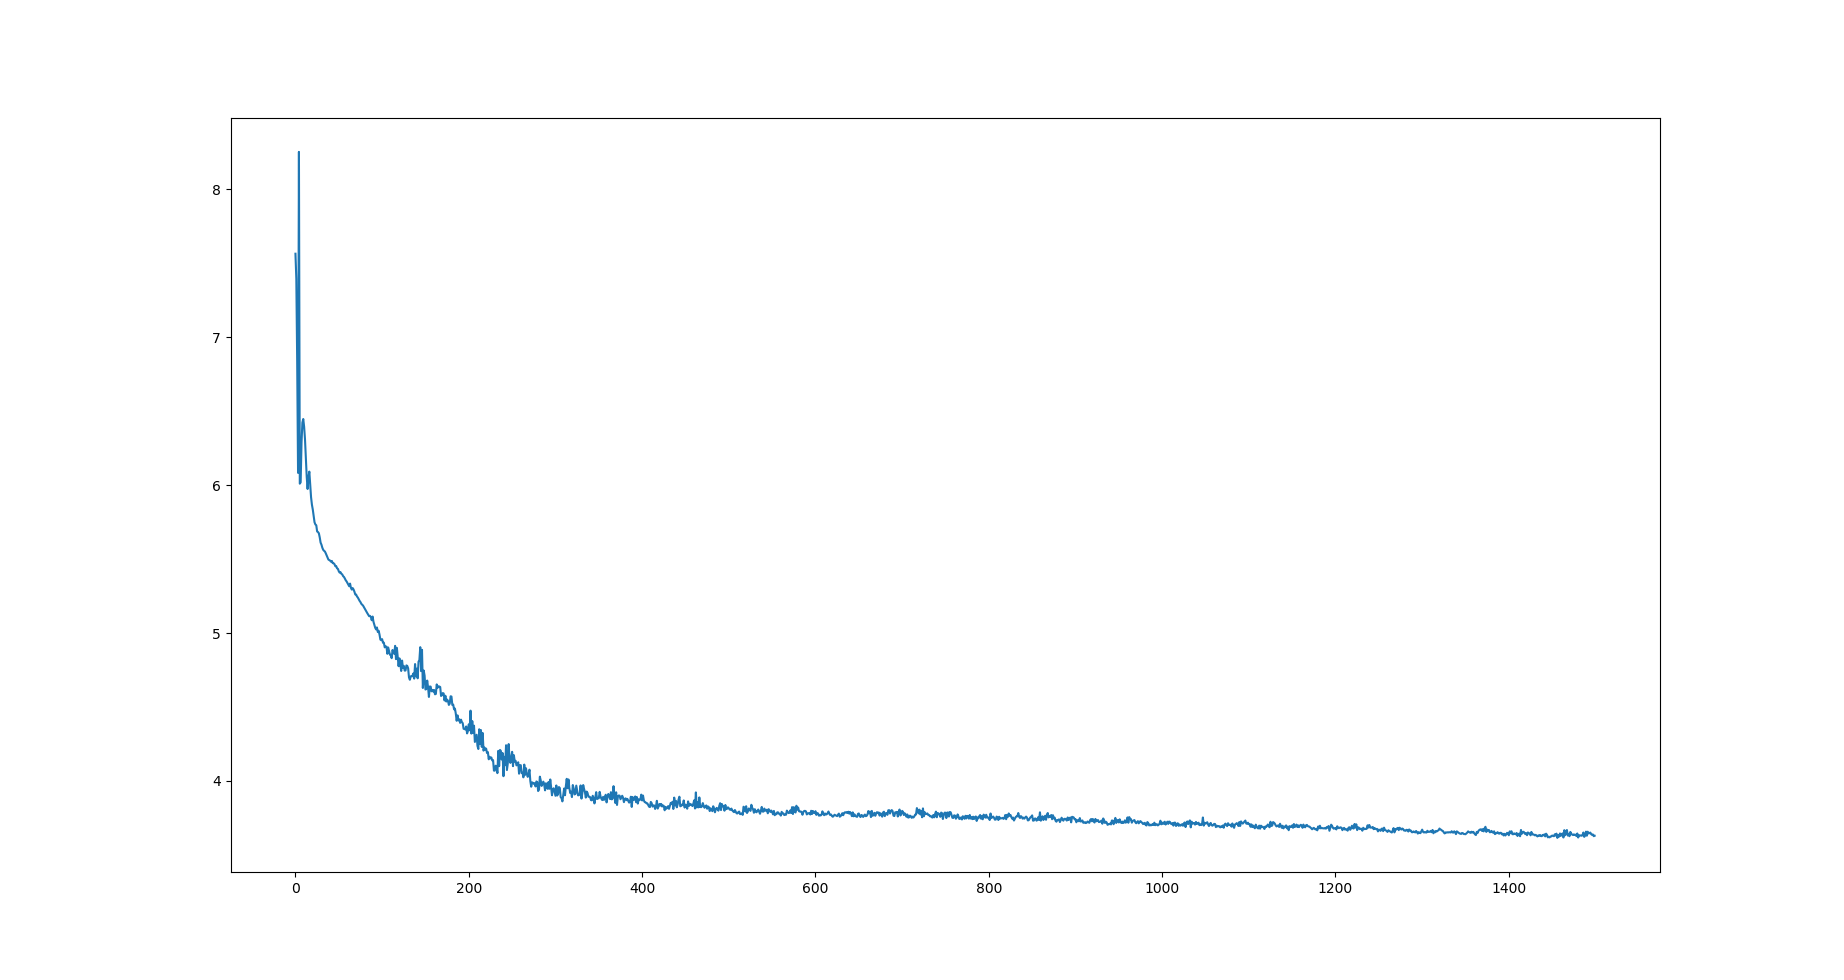
\includegraphics[width=\columnwidth]{lossIquitos}
	\caption{La reducción del error absoluto medio en cada época del entrenamiento para la ciudad de Iquitos.}
	\label{fig:lossIquitos}
\end{figure}
\begin{figure}[h]
	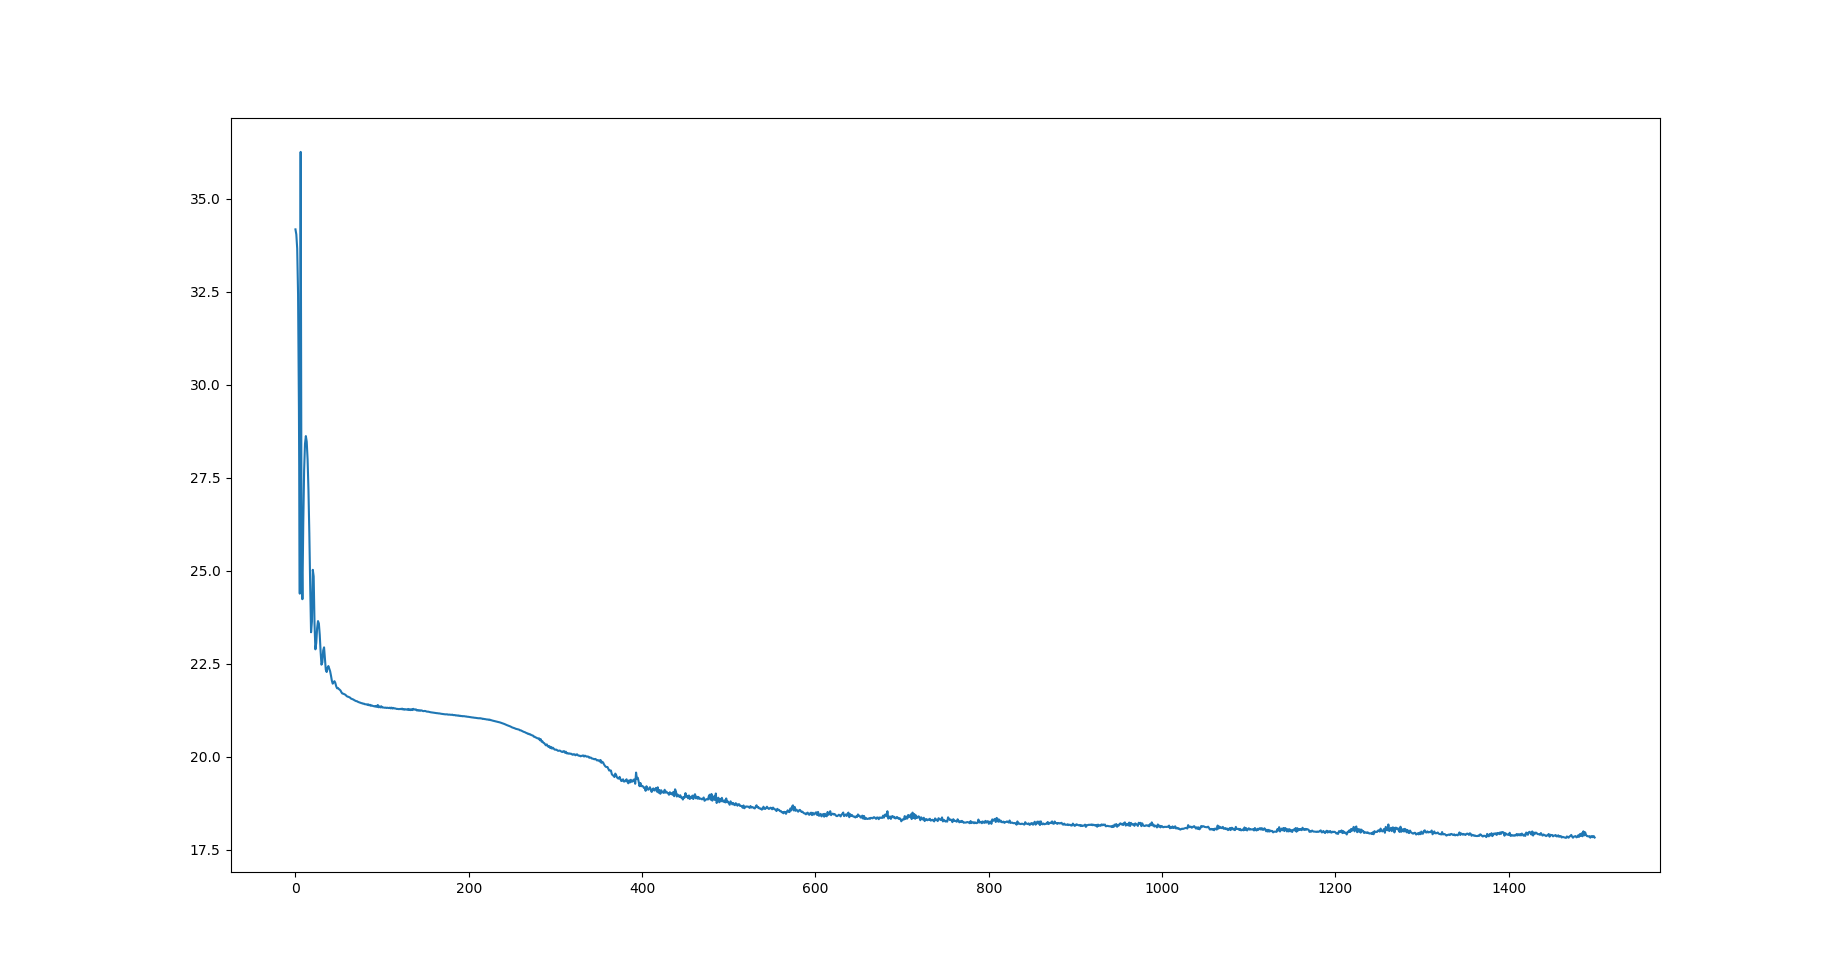
\includegraphics[width=\columnwidth]{lossSanJuan}
	\caption{La reducción del error absoluto medio en cada época del entrenamiento para la ciudad de San Juan.}
	\label{fig:lossSanJuan}
\end{figure}
Las primeras iteraciones para encontrar los parámetros que llevaban a la mejor solución se realizaron mediante el script de validación, sin embargo, para terminar de afinar los parámetros se lanzaron diversas pruebas a la competición.

\section{Aproximaciones fallidas}
Se han llevado a cabo muchas aproximaciones hasta llegar al mejor resultado. A continuación se habla de algunas de ellas.
\subsection{Eliminar filas con datos faltantes}
En lugar de interpolar o rellenar los datos faltantes utilizando la media, se optó a probar por eliminar las filas a las que les faltaban datos. Esto supuso peores resultados y se cree que es debido a la naturaleza temporal de los datos.

\subsection{Teniendo en cuenta el carácter temporal de los datos}
Se pensó también en tener en cuenta la temporalidad de los datos mediante diversas herramientas, sin embargo todas otorgaron peores resultados.
\begin{itemize}
	\item \textbf{Suavizado exponencial}: El suavizado exponencial permite añadir información de todas las situaciones anteriores a una situación determinada, de manera que, las más recientes tendrán más peso que las más antiguas. El suavizado exponencial se define así: \\
	$f(x_0,\alpha)=x_0$\\
	$f(x_t,\alpha)=x_t \cdot \alpha+(1-\alpha)\cdot f(x_{t-1},\alpha)$
	
	Este suavizado está definido con la función exponential\_smoothing en el fichero funciones.py.
	
	\item \textbf{Suavizado promediando mediante ventanas}: Este suavizado consiste en coger una ventana desde un dato hacia n datos previos y calcular el promedio de esos elementos. Este suavizado está definido con la función mean\_smoothing en el fichero funciones.py.
	
	\item \textbf{Redes neuronales recurrentes}: Las redes neuronales recurrentes son un tipo de red que ``recuerda'' entradas previas a la red y las utiliza como parte de la entrada. Se ha probado a usar un tipo de red neuronal recurrente específica: LSTM. Keras permite introducir capas especiales dentro de la red y para probar este tipo de red neuronal se introdujo una capa LSTM en la entrada del algoritmo. En el fichero scriptLSTM.py se puede ver la prueba que se hizo con una red neuronal recurrente.
\end{itemize}
Probablemente, mediante el acercamiento correcto sea posible mejorar los datos teniendo en cuenta datos anteriores, sin embargo, no ha logrado llegar a ese acercamiento.

\subsection{Suavizado temporal del número de casos para buscar patrones generales}
También se intentó entrenar el modelo, pero modificando los casos reales predichos. La forma en la que se modificó fue aplicando funciones para suavizar la evolución temporal de los casos totales de dengue. La función que se aplicó para suavizar fue el filtro de la mediana (proporcionado por la librería scipy) y se probó a aplicar ventanas de 3 y 5 elementos, pero tampoco mejoraron los resultados. 

\section{Conclusiones y problemas encontrados}

Entre los problemas encontrados cabe destacar que, debido a la inicialización aleatoria de los pesos de las redes neuronales, se han dado muchos casos en los desde el principio del entrenamiento los modelos convergían hacia mínimos locales. Para tratar con este problema lo que se ha hecho es dejar activa la opción ``verbose'' para ver cómo iba convergiendo la red y, en el caso de tomar siempre el mismo valor exacto se asumía que había convergido hacia un mínimo local y se paraba y reiniciaba la ejecución del algoritmo. Se probó también a establecer una inicialización de pesos constante, pero tendía siempre a converger hacia los mínimos locales. En relación al problema de la convergencia y de los pesos otro problema es que a veces convergía mucho más rápido y hacia valores notoriamente más pequeños que otras,. 

Si no se hubiesen tenido intentos limitados, se podrían haber obtenido mejores resultados mucho más rápido, ya que cada vez que se querían probar nuevos acercamientos era necesario esperar un día.

Otra idea que se ha barajado, pero que no se ha llevado a cabo por falta de tiempo y por la limitación de intentos es parametrizar de manera diferente el modelo de cada una de las ciudades.

Mediante la realización de este trabajo ha sido necesario aprender en profundidad el funcionamiento de las redes neuronales así como, parcialmente, las librerías Keras y TensorFlow. Además, debido a que se han probado muchas técnicas y acercamientos, se han adquirido conocimientos para enfocar problemas de este tipo desde perspectivas poco obvias.

\end{document}
